At the end of this worksheet you should be able to  

\begin{itemize}
	\item discuss Newton's laws and provide examples of the application of each.
	\item apply Newton's first law to solve interesting physical problems.
	\item apply Newton's second law to solve interesting physical problems for objects that accelerate.
	\item apply Newton's third law to situations involving the motion of multiple objects. 


\end{itemize}


\begin{enumerate}
\setlength\itemsep{1 in}

% \item What is the difference between mass and weight? Why can we use them interchangeably at the grocery store?

\item What base units are the composite force units of Newtons equal to?

% \item What is the force of gravity between the moon and the earth? You will need to look up some values.

% \item What is the force of gravity between two \SI{75}{\kilogram} people standing 1m apart?\bigskip

% \item Find the radius from the center of the earth where Earth's gravitational field strength would 

% \begin{itemize}
%	\item $\tfrac{1}{2}$ of its value at the surface.
%	\item $\tfrac{1}{3}$ of its value at the surface.
%	\item What would be the \emph{altitude} where the gravitational field is $\tfrac{1}{4}$ its value at the surface?
%	\item What is the gravitational field strength at the altitude that the space station orbits the earth?
%\end{itemize}
%\hugeskip

\item
\begin{enumerate}
\item If I hold a \SI{5}{\kilogram} cup motionless in my hand, what force do I provide to the cup?\hugeskip
\item If I raise a \SI{5}{\kilogram} cup with my hand, \emph{at constant speed}, then what force do I need to provide from my hand to the cup?\hugeskip
\item If I accelerate the cup upwards with an acceleration of \SI{+1}{\meter \per \second^2}, then what force does my hand need to provide to the cup?\hugeskip

\item If I accelerate the cup downwards with an acceleration of \SI{-1}{\meter \per \second^2}, then what force does my hand need to provide to the cup?\hugeskip
\end{enumerate}


\item If I push a \SI{100}{\kilogram} box with an applied force of \SI{700}{\newton} along a friction-less surface. Find the force of gravity on the box, the normal force, and the net force.\hugeskip

\item Take the same problem from above and now add friction. The coefficient of friction is $\mu=0.5$ then what is the net force?\hugeskip

\item For both of the previous problem, what happens when I stop pushing?

\item What force do I need to exert to push the box at constant speed?

% \item In order to keep a box moving \emph{at constant speed} along a friction-less level surface, what pushing force is required?\\
% \item If I have to exert a force to keep a box moving along a level surface at constant speed, then what other force is probably present? What is the net force on the box in this case?\\

\item If I need to provide a \SI{1000}{\newton} force to keep a \SI{100}{\kilogram} box moving at constant speed along a level floor, then what is the coefficient of friction between the floor and the box?\hugeskip

\item A \SI{1000}{\kilogram} car is parked on a hill that has an angle of \ang{10} with respect to the horizontal. What is the weight of the car? What is the normal force on the car? What force is keeping the car from sliding down the hill? How large is that force?\giantskip

\item If the maximum incline that the car can be parked on without sliding is \ang{25}, then what is the coefficient of friction between the tires and the road?\giantskip

\item Work the previous problem inside-out.\giantskip

\item A 100 kg box slides down a friction-less inclined plane that has an angle of \ang{30} to the horizontal. What is the net force on the box and then what is the acceleration of the box?
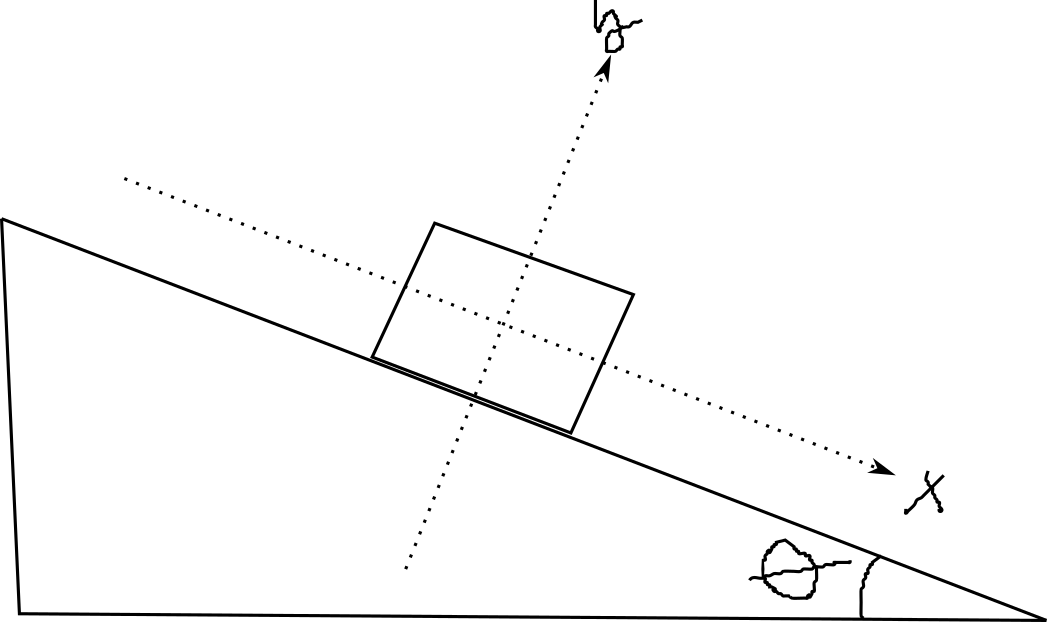
\includegraphics[scale=0.75]{week-3-incline-plane.png}
\bigskip

\item A 100 kg box slides down a friction-full inclined plane that has an angle of \ang{30} to the horizontal and a coefficient of friction of $\mu=0.1$. What is the net force on the box and then what is the acceleration of the box?\giantskip

\item Let's do the friction-less inclined plane problem \emph{in general} for any mass and incline. Follow the same procedure as before but with the variable $m$ for mass and $\theta$ for incline angle. Find an expression for the net force on the mass as a function of $\theta$ and for the acceleration as a function of $\theta$.\giantskip 

\item Now let's do the inclined plane with friction \emph{in general}. Just like the previous problem, use $m$ for mass, $\theta$ for angle, and now use $\mu$ as a variable for coefficient of friction. Find an expression for the acceleration of the mass as a function of $\theta$, $m$, and $\mu$. \giantskip

\item In order to \emph{hold} a box on a friction-less inclined plane, that is kept motionless, what force would be necessary to do that? Is there a difference between the force to hold it motionless on the incline and the force to push it up the incline \emph{at constant speed}? \giantskip

%%\needspace{5\baselineskip}
%\item An 80kg person is pulling on a string tied to a wall with a force of 100N. What is the tension measured in the string?
%
%
%\item An 80kg person is pulling on a string with a 100N force against a 60kg person. Both people are at rest. What is the tension in the string?

\item A \SI{50}{\kilogram} weight is suspended in three different ways shown below. What is the tension in each rope?

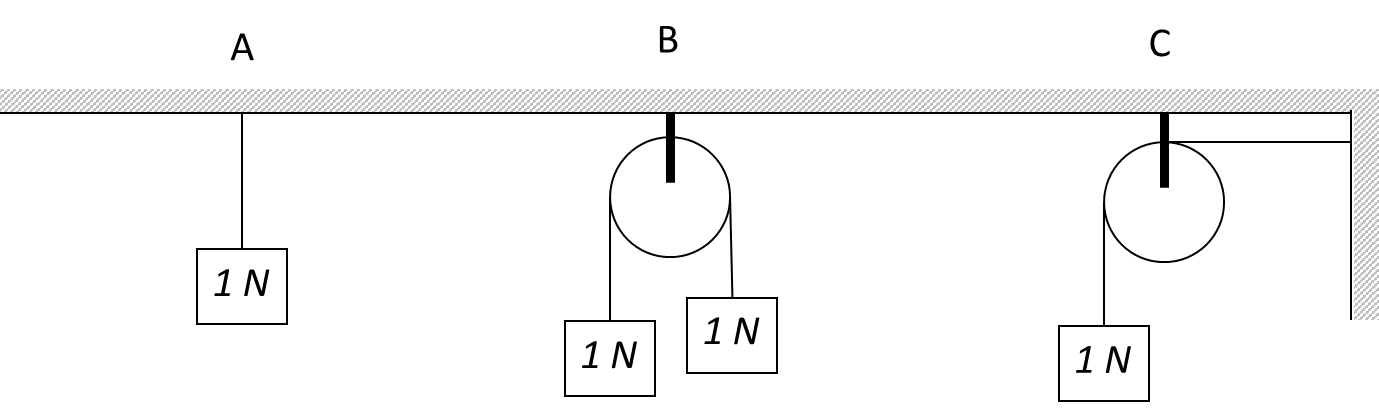
\includegraphics[scale=.70]{3separatePulleys.png}\bigskip

\item I am pulling two objects connected by a string. They are both \SI{100}{\kilogram}. There is no friction between the objects and the surface, and they are accelerating at \SI{1}{\meter/\second^2}. What is my pulling force and what tension force is between the boxes? \giantskip


\item One object $m_1$ connected by a string to another object $m_2$ that is hanging off the edge of the table. There is a pulley at the edge of the table so the string is not introducing any friction to the system. If this is a friction-less table, then what is an expression for the acceleration of the objects?\giantskip

%\needspace{5\baselineskip}
\item Now do the previous problem again, but with a coefficient of friction $\mu$ between the sliding mass ($m_1$) and the surface.


%
%\item
%What is a displacement? What is velocity? What is acceleration? How do you know you have moved places or how do you know you are in motion? How do you know you are accelerating?\bigskip
%
%
%\item If I go from $x=\SI{10}{\meter} $ to $ x=\SI{28}{\meter}$, then what is my displacement? If it takes 12 seconds to do that, then what is my average velocity over that interval. Does this mean that my velocity has this value at every instant along the path?\bigskip
%
%\item If I am initially going \SI{+10}{\meter / \second} and it takes me 15 seconds to speed up to  \SI{+25}{\meter/ \second}, then what is my acceleration?\bigskip
%
%\item If my acceleration is \SI{+10}{\meter / \second^2}, then if I started at rest, how long would it take me to speed up to \SI{+45}{\meter /\second}? How fast would I be going after 10 seconds?\hugeskip



\end{enumerate}